\documentclass[12pt, letterpaper]{article}
\usepackage{graphicx} % Required for inserting images
\usepackage{hyperref}
\usepackage{listings}
\usepackage{amssymb}
\usepackage{amsmath}
\usepackage[english]{babel}
\usepackage{nicefrac, xfrac}
\usepackage{mathtools}
\newcommand{\acc}{\\\hphantom{}\\}
\usepackage[table,xcdraw]{xcolor}
\usepackage[paper=a4paper,left=20mm,right=20mm,bottom=25mm,top=25mm]{geometry}
\renewcommand{\labelenumii}{\arabic{enumi}.\arabic{enumii}}
    \renewcommand{\labelenumiii}{\arabic{enumi}.\arabic{enumii}.\arabic{enumiii}}
    \renewcommand{\labelenumiv}{\arabic{enumi}.\arabic{enumii}.\arabic{enumiii}.\arabic{enumiv}}
\title{Università 2 (gruppo 42)}
% \author{ Giacomo Biribicchi \and Marco Casu \and Christian Di Manno \and Alessandro Gautieri }
\date{}


\begin{document}

\maketitle


\section{Requisiti}
I dati di interesse per il sistema sono \underline{Studenti}, \underline{Facoltà}, \underline{Professori} e \underline{Corsi}.
\begin{enumerate}
    \item \textbf{Studente}\begin{enumerate}
        \item nome e cognome
        \item codice fiscale 
        \item matricola 
        \item data di nascita 
        \item città di nascita 
        \item corso di laurea - Il/I corso/corsi alla quale lo studente è iscritto.
        \item insegnamenti superati - Gli \underline{Insegnamenti} che lo studente ha superato, uno stesso \underline{Insegnamento} non può essere 
        superato più di una volta.
    \end{enumerate}
    \item \textbf{Professore}\begin{enumerate}
        \item nome e cognome
        \item data di nascita 
        \item codice fiscale 
        \item città di nascita 
        \item insegnamenti erogati - L'\underline{Insegnamento} (o più di uno) erogato da un \underline{Professore}.
    \end{enumerate}
    \item \textbf{Corso di Laurea}\begin{enumerate}
        \item nome 
        \item facoltà
    \end{enumerate}
    \item \textbf{Facoltà}\begin{enumerate}
        \item nome
    \end{enumerate}
    \item \textbf{Insegnamento}\begin{enumerate}
        \item nome 
        \item ore di lezione 
        \item corsi alla quale appartiene - Il \underline{Corso di Laurea} nel quale un \underline{Insegnamento} viene erogato.
        \item codice -  Serie di caratteri alfanumerici che identificano univocamente un \underline{Insegnamento}.
    \end{enumerate}
\end{enumerate}
\newpage
\section{Considerazioni}
Sarebbe possibile considerare una generalizzazione delle classi  \underline{Professore} e  \underline{Studente}, denotata 
\underline{Persona}, in quanto queste due condividono più aspetti, come l'associazione ad una città, o i vari attributi identificativi,
differiscono esclusivamente nella loro relazione con \underline{Insegnamento}. Sarebbe quindi corretto considerare 
\underline{Professore} e  \underline{Studente} come \textit{sottoclassi} di \underline{Persona}.
\section{Documenti di Specifica}
\subsection{Tipi di Dato}
I tipi sono dati sottoforma di espressioni regolari : \acc
Matricola = Stringa [0-9]\{7\}\acc 
CF = [A-Z]\{6\} [0-9]\{2\} [A-Z]\{1\} [0-9]\{2\} [A-Z]\{1\} [0-9]\{3\} [A-Z]\{1\}
\section{UML}
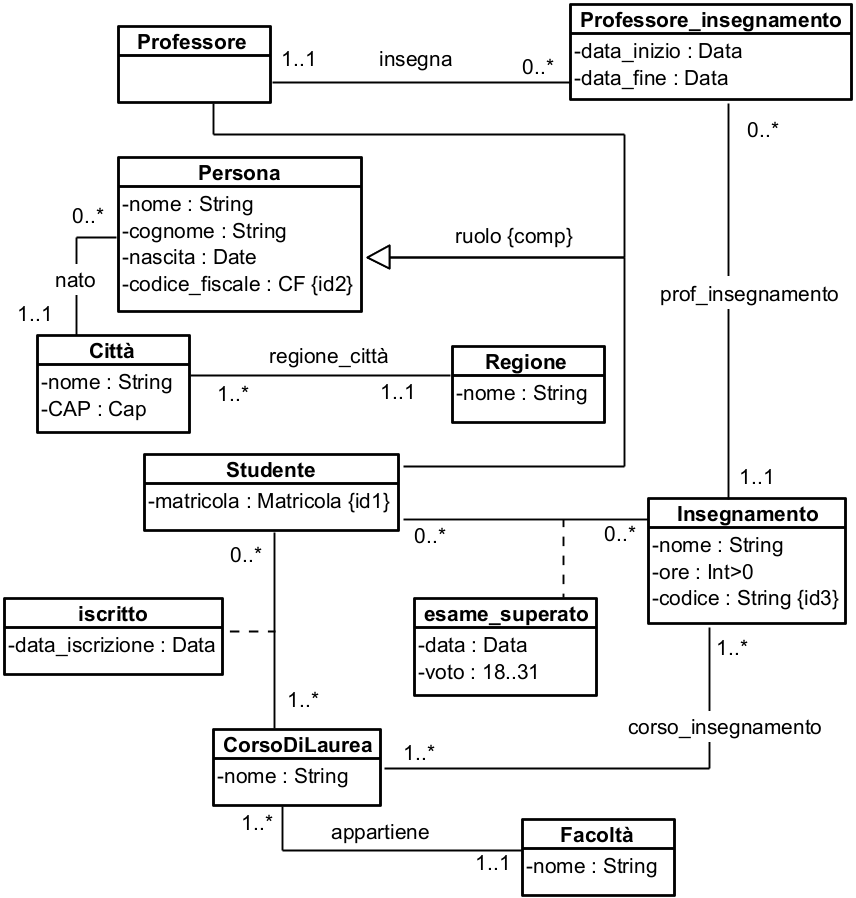
\includegraphics[width=\textwidth]{images/UML.png}


\end{document}

